\section{ListGraphVisitor.h File Reference}
\label{ListGraphVisitor_8h}\index{ListGraphVisitor.h@{ListGraphVisitor.h}}


\subsection{Detailed Description}
\begin{Desc}
\item[Author:]Troy Taillefer \end{Desc}


\begin{Desc}
\item[Date:]December 7, 2007 \end{Desc}
\begin{Desc}
\item[Version:]0.1 \end{Desc}


Definition in file {\bf ListGraphVisitor.h}.

{\tt \#include $<$boost/graph/depth\_\-first\_\-search.hpp$>$}\par
{\tt \#include $<$boost/shared\_\-ptr.hpp$>$}\par
{\tt \#include \char`\"{}SceneGraph.h\char`\"{}}\par
{\tt \#include $<$string$>$}\par
{\tt \#include $<$vector$>$}\par


Include dependency graph for ListGraphVisitor.h:\nopagebreak
\begin{figure}[H]
\begin{center}
\leavevmode
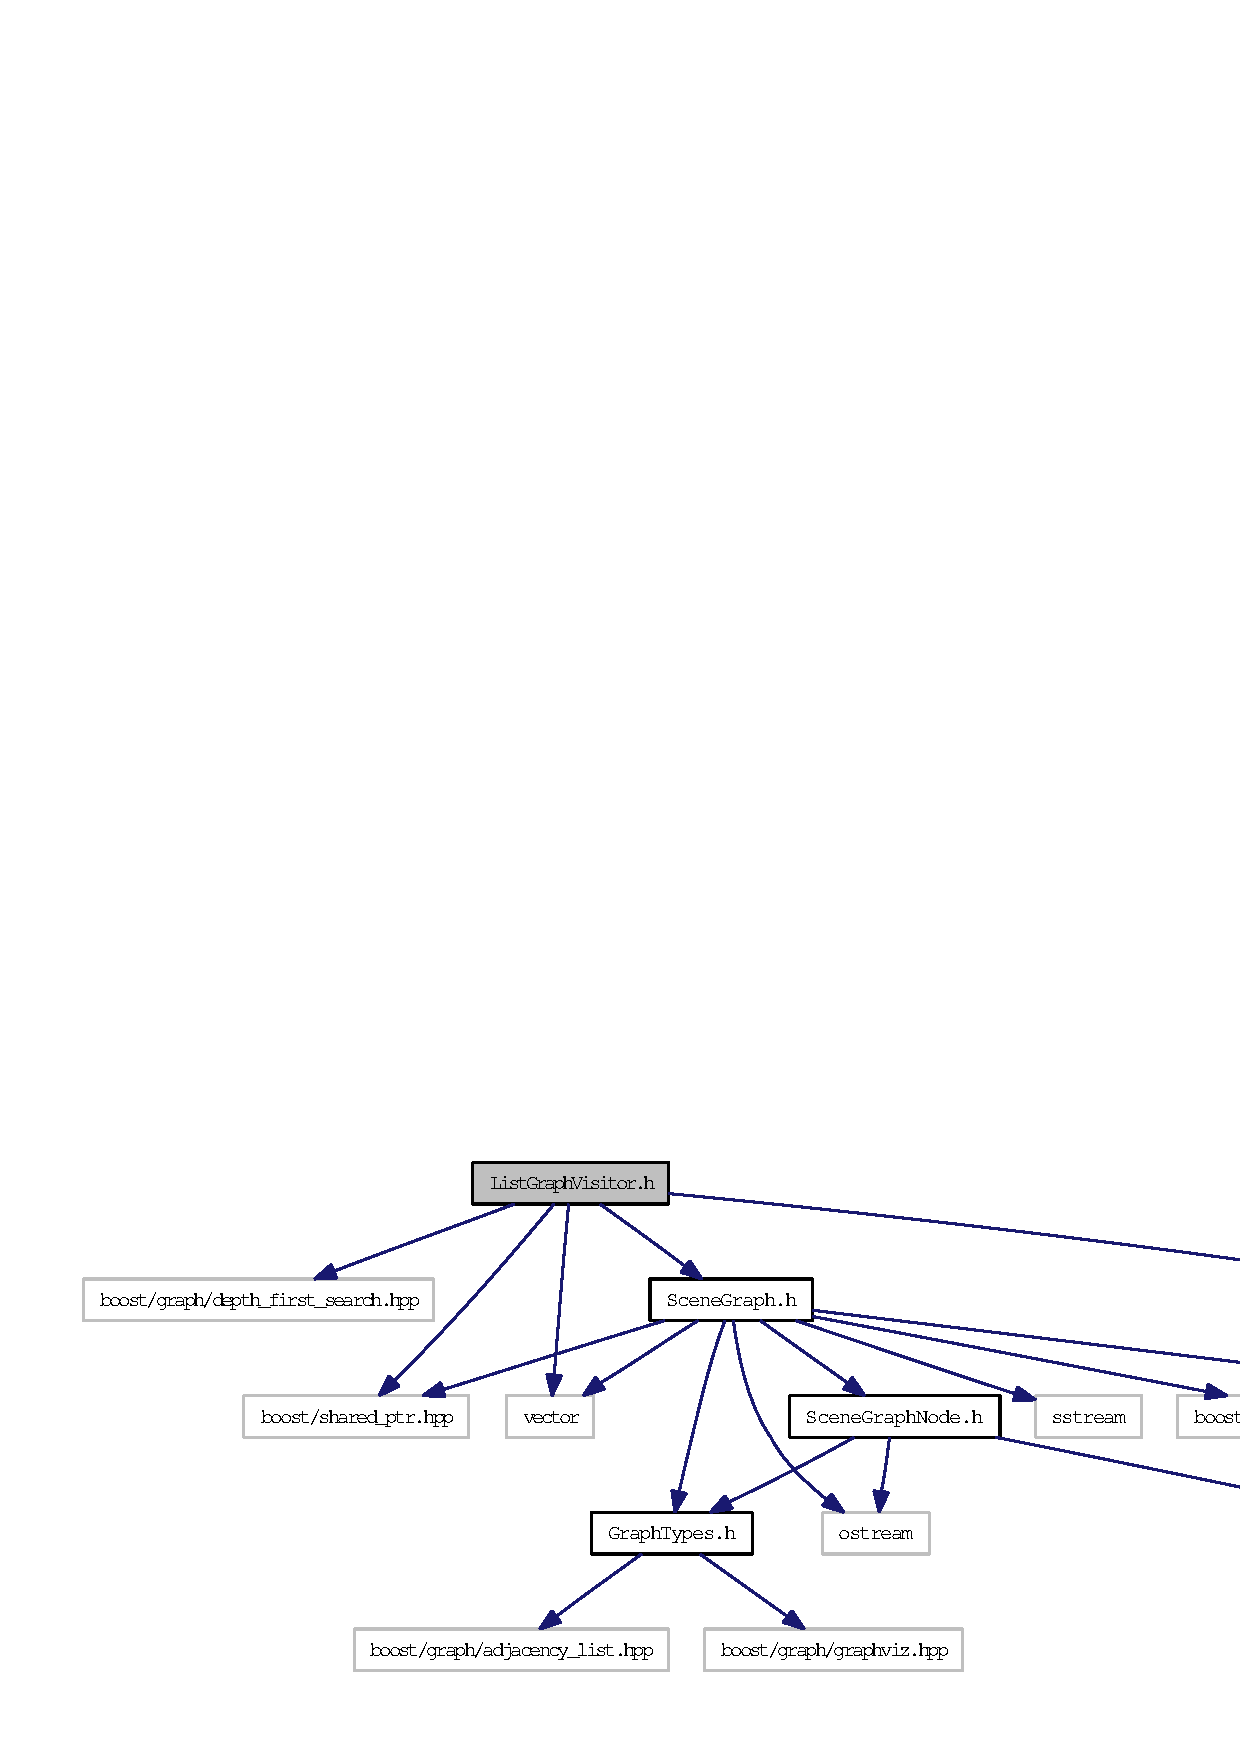
\includegraphics[width=420pt]{ListGraphVisitor_8h__incl}
\end{center}
\end{figure}


This graph shows which files directly or indirectly include this file:\nopagebreak
\begin{figure}[H]
\begin{center}
\leavevmode
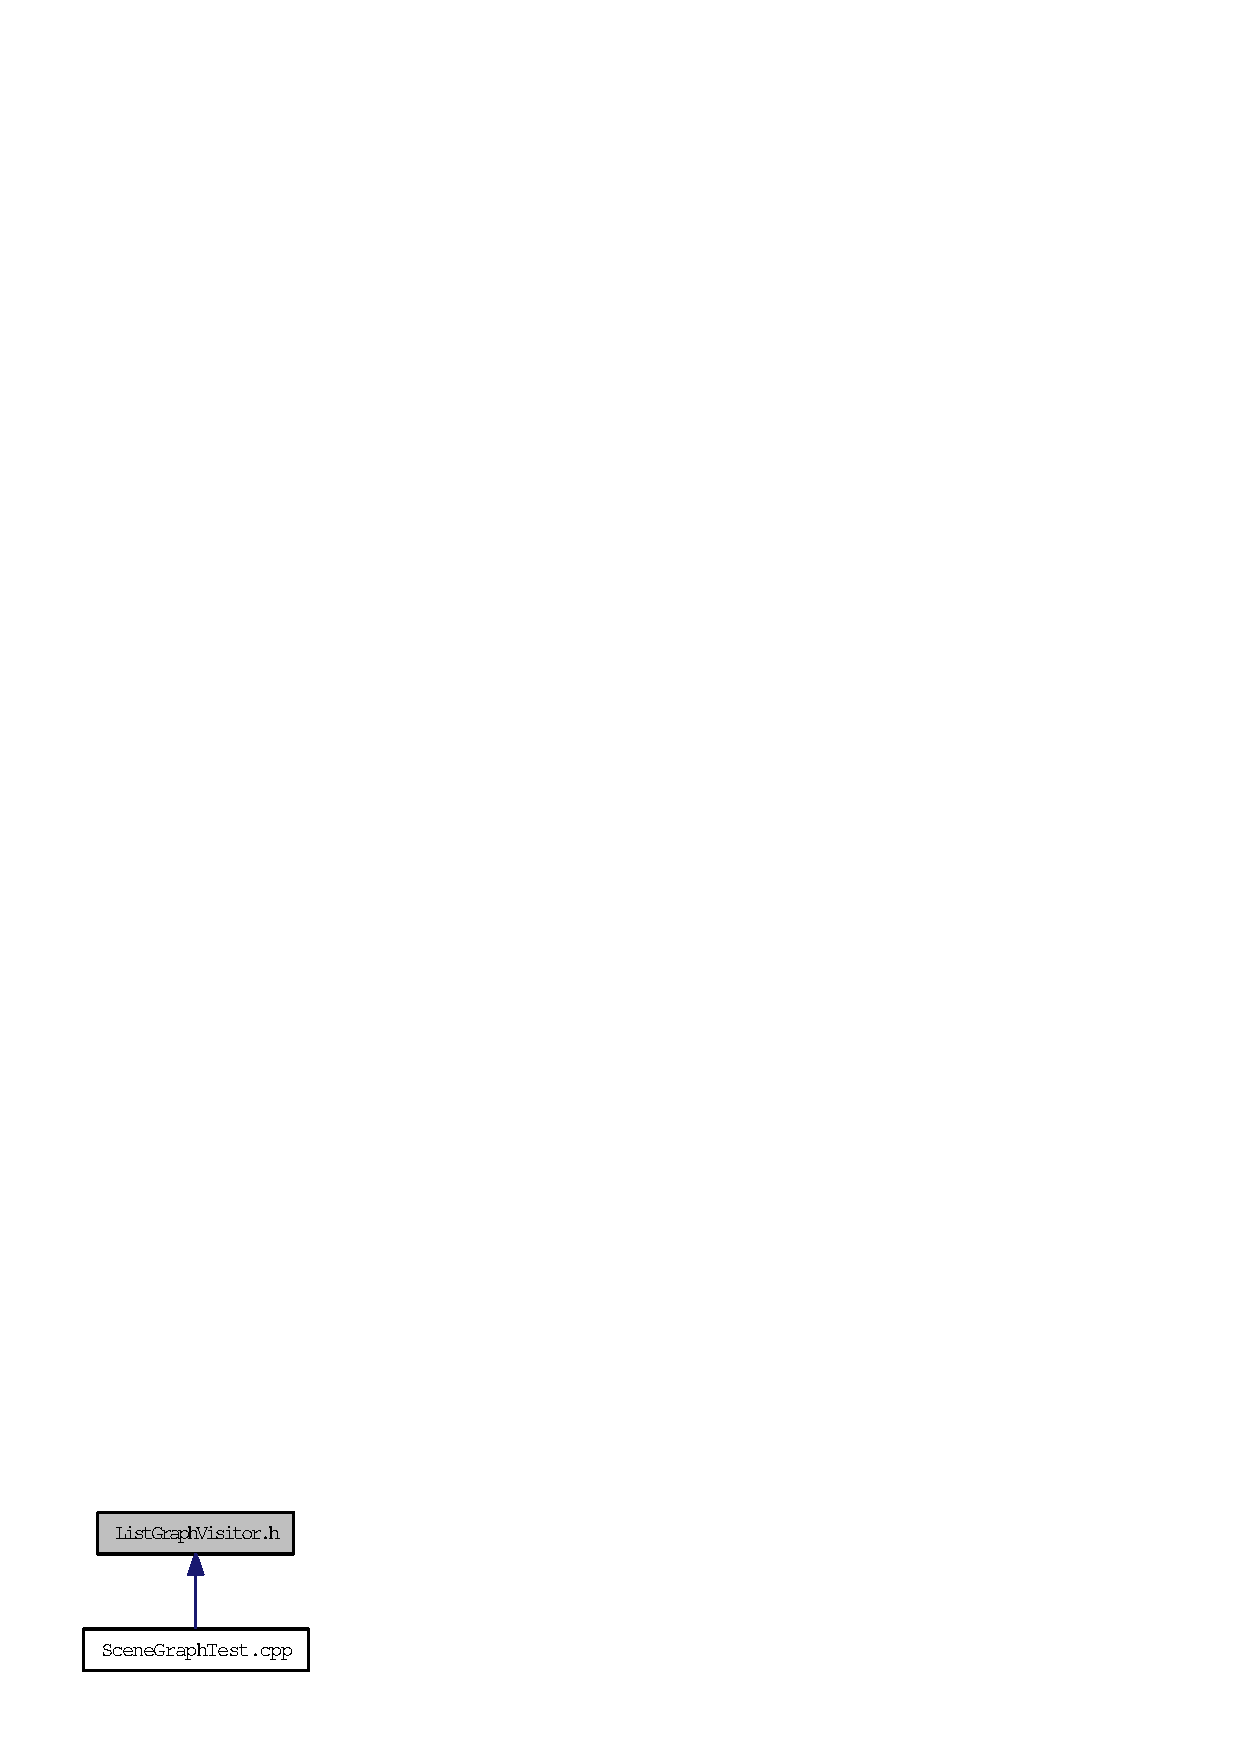
\includegraphics[width=76pt]{ListGraphVisitor_8h__dep__incl}
\end{center}
\end{figure}
\subsection*{Data Structures}
\begin{CompactItemize}
\item 
class {\bf ListGraphVisitor}
\begin{CompactList}\small\item\em This class list the node in the order they would be encountered depth first and builds a formatted string using newline and tab characters to show the structure of the graph it follows a variant of the visitor desing pattern. \item\end{CompactList}\end{CompactItemize}
